\documentclass[12pt]{article}

\usepackage[utf8]{inputenc}
\usepackage{Preambles/preamble}
\usepackage{listings}
\usepackage{url}
\usepackage{graphicx}
\usepackage{amsfonts,amsmath,oldgerm,mathtools,xeCJK}
\usepackage{xcolor}
\usepackage{graphicx}
\usepackage{hyperref}
\usepackage{biblatex}

\lstset{
  language=Python,
  caption={},frame=single, backgroundcolor=\color{gray!10}, basicstyle=\footnotesize, framexleftmargin=3pt, commentstyle=\color{mygreen},
  keywordstyle=\color{blue},
  stringstyle=\color{red},
  identifierstyle=\color{darkgreen},
  numbers=left,
  numberstyle=\tiny\color{gray},
  frame=single,
  rulecolor=\color{black},
  breaklines=true,
  showstringspaces=false,
  captionpos=b,
  escapeinside={(*@}{@*)}, % allows you to add LaTeX within your code
}


%~~~~~~~~~~~~~~~~~~~~~~~~~~~~~~~~~~~~~~~~~~~~~~~~~~~~~~~~~~~~~~
\begin{document}

\title{Project report: Coupling ScimBa and Feel++}

\firstauthor{Helya Amiri}
\firstemail{helya.amiri@etu.unistra.fr}
\secondauthor{Rayen Tlili}
\secondemail{rayen.tlili@etu.unistra.fr}
\supervisor{Christophe Prud'homme, Joubine Aghili}
\submitdate{\today}
\maketitle

\addtocounter{page}{-1}
\pagenumbering{roman}
\thispagestyle{empty}


\newpage
\doublespacing
\tableofcontents
\singlespacing
%~~~~~~~~~~~~~~~~~~~~~~~~~~~~~~~~~~~~~~~~~~~~~~~~~~~~~~~~~~~~~~
%Sections before Main Content of report

\newpage
\section*{Abstract}\label{Conventions}
\addcontentsline{toc}{subsection}{\textit{Abstract}}
\begin{frame}
    This project report the details of the integration efforts between ScimBa, emphasizing machine learning, and Feel++, known for its Galerkin methods in PDE solving. The aim is to establish a wrapper between the two libraries combining machine learning with traditional PDE solvers.
    
\end{frame}
\vspace{2em}

%~~~~~~~~~~~~~~~~~~~~~~~~~~~~~~~~~~~~~~~~~~~~~~~~~~~~~~~~~~~~~~
%Main Content sections start

\newpage
\pagenumbering{arabic}
\section*{Main Content}
\addcontentsline{toc}{part}{Main Content}

\section{Introduction} \label{Sec: Introduction}

A wrapper is a design pattern or a piece of code that serves as an intermediary between other code components. This report presents the objectives, approach, and roadmap for the wrapping of ScimBa and Feel++ libraries. 


\subsection{Objectives}

\begin{enumerate}
    \item \textbf{Streamlined Data Exchange}: Develop a system that streamlines data exchange between ScimBa and Feel++, enabling seamless interaction between the two libraries.
    
    \item \textbf{User Empowerment}: Create an interface that allows users to leverage the combined tools of ScimBa and Feel++ effectively.
    
    \item \textbf{Integration of Technologies}: Integrate various technologies such as Docker, Python, and Git to create a reproducible environment for the project, apply machine learning techniques, solve PDEs, and manage source code.
    
    \item \textbf{Add necessary files and dependencies to ScimBa and Feel++}: Contribute to both projects by offering users a platform that unifies machine learning techniques and PDE solving methods to work with and compare.
\end{enumerate}

Once the proper environment has been set up in the docker image, we started working on a program that will solve various PDEs using the Feel++ method and the Scimba method to visualize and compare the results.


\begin{enumerate}
    \item \textbf{Generate multiple results using Feel++ toolboxes}: Using the CFDE toolbox to solve Poisson equations with varying parameters and visualizing them on varying geometries.
    
    \item \textbf{Understanding and exporting results using ScimBa}: Explore the ScimBa repository and use examples from Pinns (Physics-informed neural networks) to solve a Poisson equation and visualize the results.
    
    \item \textbf{Creating a program that is able to use both as solvers}: One of the primary objectives to reach for this project is to create a program that is able to call upon the Feel++ CFPDE toolbox and the ScimBa machine learning algorithms to solve various PDEs.
    
    \item \textbf{Comparing the results of both solvers}: The results of both solvers will be able to be visualized and compared in terms of efficiency and accuracy.

    \setcounter{enumi}{4}
    \item \textbf{Expand Application Scope}: After successfully solving Poisson equations, expand the application of the program to solve other types of PDEs, further demonstrating the versatility of the integrated system.
    
    \item \textbf{Optimize Performance}: Continually optimize the performance of the program, ensuring that it runs efficiently and effectively on various hardware configurations.
    
    \item \textbf{User-Friendly Interface}: Develop a user-friendly interface that allows users with varying levels of technical expertise to utilize the program effectively.
    
    \item \textbf{Documentation and Training}: Provide comprehensive documentation and training materials to help users understand how to use the program and interpret the results.
    
    \item \textbf{Community Engagement}: Engage with the user community to gather feedback, identify areas for improvement, and guide future development efforts.
\end{enumerate}



\subsection{Roadmap}  
\label{sec:Roadmap}

\begin{frame}

\begin{enumerate}
    \item Explore Feel++ and ScimBa documentation.
    \item Create a container using docker with a Feel++ base and install ScimBa within it.
    \item Solve PDEs using Feel++.
    \item Solve PDEs using ScimBa PINNs.
    \item Create a Poisson class you can call to solve using Feel++.
    \item Add ScimBa as a solver for the class by updating the Poisson2d class to handle ScimBa with parametrized f, g and add a diffusion tensor to the Poisson2d class.
    \item Compare the results of both solvers with exact solutions.
    \item Compute \( L^2\) and \( H^1 \) errors and trace their convergence for both solvers.
\end{enumerate}
\end{frame}

    
%~~~~~~~~~~~~~~~~~~~~~~~~~~~~~~~~~~~~~~~~~~~~~~~~~~~~~~~~~~~~~~
\newpage 


\section{Exploring Feel++ documentation}
First, both of us explored the Feel++ toolboxes on our own.
Feel++ is a library that allows manipulation of mathematical objects to solve Partial Differential Equations (PDEs). It also provides toolboxes for physics-based models and their coupling. These toolboxes include applications for:

\begin{itemize}
    \item Fluid mechanics
    \item Solid mechanics
    \item Heat transfer and conjugate heat transfer
    \item Fluid-structure interaction
    \item Electro and magnetostatics
    \item Thermoelectrics
    \item Levelset and multifluid
\end{itemize}


\subsection{Exploring Feel++ toolboxes}

As of the first meeting with the project supervisors, we've taken a look at the different toolboxes Feel++ has to offer in Python:
\begin{frame}{}
    \begin{center}
        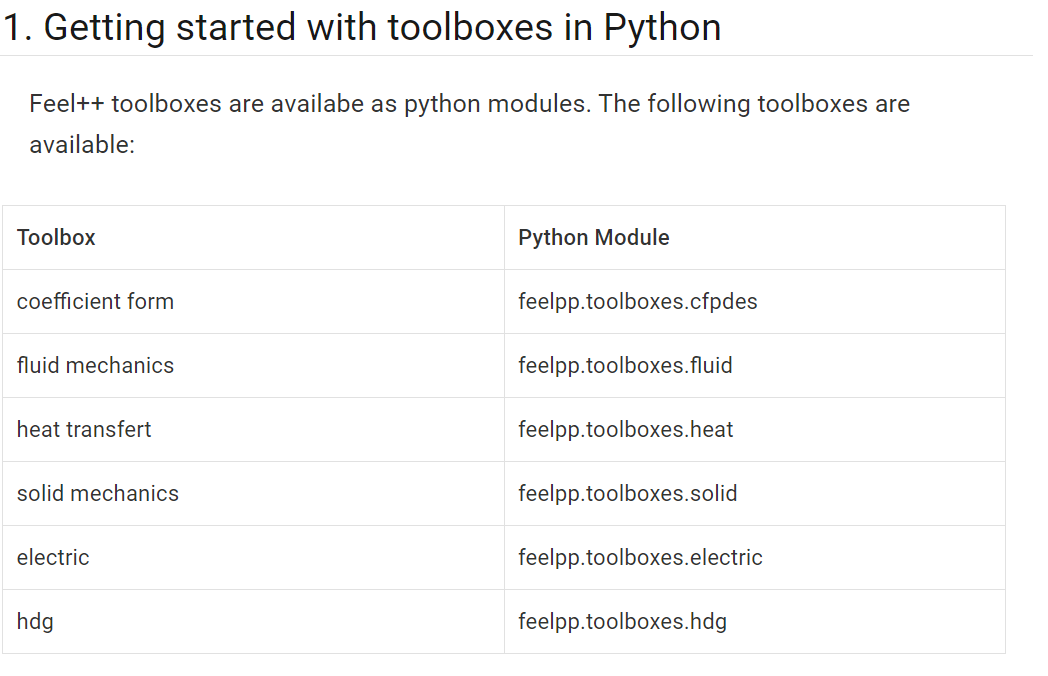
\includegraphics[width=6in]{images/pyfeelpptoolboxes.png}
    \end{center}
\end{frame}

An interesting toolbox to start with is the \textbf{Coefficient Form PDEs}:

%~~~~~~~~~~~~~~~~~~~~~~~~~~~~~~~~~~~~~~~~~~~~~~~~~~~~~~~~~~~~~~
\subsection{Coefficient Form Toolbox}

\begin{enumerate}
    \item \textbf{What are Coefficient Form PDEs?}: The coefficient forms in PDE (Partial Differential Equation) toolboxes encapsulate crucial properties like diffusion, convection, and reaction coefficients. These coefficients are vital for characterizing diverse PDEs such as elliptic, parabolic, or hyperbolic equations, each with its unique coefficient form.
    For instance, in the Poisson equation, a common elliptic equation, the coefficient form is often expressed as:
    \[
        -\nabla \cdot (c \nabla u) + au = f
    \]

    \begin{itemize}
        \item \(c\) : represents the diffusion coefficient,
        \item \(a\) : represents the reaction coefficient,
        \item \(u\) : is the unknown function, and
        \item \(f\) : is the source term.
    \end{itemize}
    
    PDE toolboxes, such as Feel++, offer features for handling different PDEs. They make it easier to define coefficients, set boundaries, discretize problems, and use numerical methods. This helps users to solve complex PDEs, study physical phenomena, and simulate real-world situations more efficiently.

    \item \textbf{System of PDEs}: Many PDEs can be expressed in a standard form, mainly based on the coefficients' definition. We use the following equation to find this form: \\
    \( u \) : \( \Omega \subset \mathbb{R}^d \longrightarrow \mathbb{R}^n \) with \( d = 2, 3 \) and \( n = 1 \) ( \( u \) is a scalar field) or \( n = d \) ( \( u \) is a vector field) such that
    \[
    d \frac{\partial u}{\partial t} + \nabla \cdot \left( -c \nabla u - \alpha u + \gamma \right) + \beta \cdot \nabla u + au = f \text{ in } \Omega
    \]
    \begin{itemize}
        \item \( d \) : damping or mass coefficient
        \item \( c \) : diffusion coefficient
        \item \( \alpha \) : conservative flux convection coefficient
        \item \( \gamma \) : conservative flux source term
        \item \( \beta \) : convection coefficient
        \item \( a \) : absorption or reaction coefficient
        \item \( f \) : source term
    \end{itemize}
    Parameters \( \mu \) may depend on the unknown \( u \) and on the space variable \( x \), time \( t \), and other unknowns \( u_1, \ldots, u_N \).
%~~~~~~~~~~~~~~~~~~~~~~~~~~~~~~~~~~~~~~~~~~~~~~~~~~~~~~~~~~~~~~
\newpage

    \item \textbf{Coefficients}: We also need to follow certain limitations on coefficient shapes, as detailed in the table below.
    \begin{figure}[H]
    \centering
    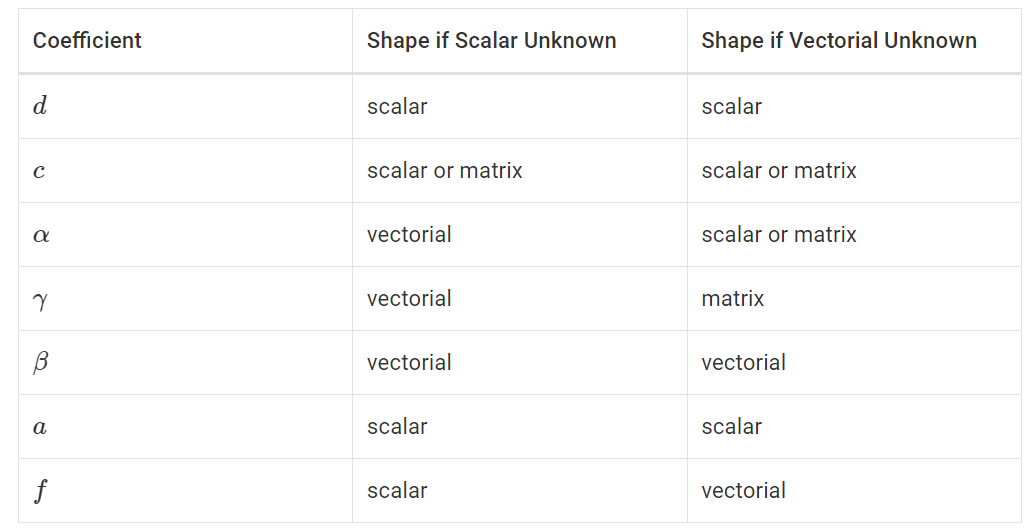
\includegraphics[width=7in]{images/coeff.png}
    \captionsetup{font={scriptsize}}
    \caption{Shape required by the coefficients}
    \end{figure}
    
    \item \textbf{Initial Conditions}: Initial Initial conditions set the initial values for each unknown variable in the equations. These conditions can be defined using expressions or fields.
    
    \textbf{ Boundary Conditions}: 
    \begin{itemize}
        \item Dirichlet
        \item Neumann
        \item Robin
    \end{itemize}
    
 
\end{enumerate}



%~~~~~~~~~~~~~~~~~~~~~~~~~~~~~~~~~~~~~~~~~~~~~~~~~~~~~~~~~~~~~~
\newpage

\section{Getting familiar with ScimBa}

We decided to start using the examples in the ScimBa repository of uses of the Physics-Informed Neural Networks (PINNs). PINNs integrate the underlying physical laws described by PDEs directly into the learning process of neural networks. This is achieved by constructing a loss function that penalizes the network for failing to fit known data and for violating the given physical laws.

\begin{lstlisting}
from lap2D_pinns import Run_laplacian2D, Poisson_2D
from scimba.equations import domain


# Define a square domain
xdomain = domain.SpaceDomain(2, domain.SquareDomain(2, [[0.0, 1.0], 
                                                    [0.0, 1.0]]))

# Create an instance of the Poisson problem
pde = Poisson_2D(xdomain)

# Run the training
Run_laplacian2D(pde)

\end{lstlisting}

The class Poisson 2D is initialized with a given spatial domain (space domain) and sets up the problem with one unknown variable and one parameter.
The parameter domain is narrowly defined, likely to enforce precise boundary conditions or to stabilize the solution.
\begin{lstlisting}
class Poisson_2D(pdes.AbstractPDEx):
    def __init__(self, space_domain):
        super().__init__(
            nb_unknowns=1,
            space_domain=space_domain,
            nb_parameters=1,
            parameter_domain=[[0.50000, 0.500001]],
        )

\end{lstlisting}


The Run laplacian2D function encapsulates the entire process of setting up, training, and evaluating a neural network to solve the Laplacian PDE using PINN. This includes data sampling, network configuration, loss calculation, and optimization.

\begin{lstlisting}

def Run_laplacian2D(pde, bc_loss_bool=False, w_bc=0, w_res=1.0):
    x_sampler = sampling_pde.XSampler(pde=pde)
    mu_sampler = sampling_parameters.MuSampler(
        sampler=uniform_sampling.UniformSampling, model=pde
    )
    sampler = sampling_pde.PdeXCartesianSampler(x_sampler, mu_sampler)

\end{lstlisting}
\\
We will talk further about the files and visuals generated in both cases in the "Results" section.

Other neural networks available on ScimBa:

\begin{figure}[H]
    \centering
    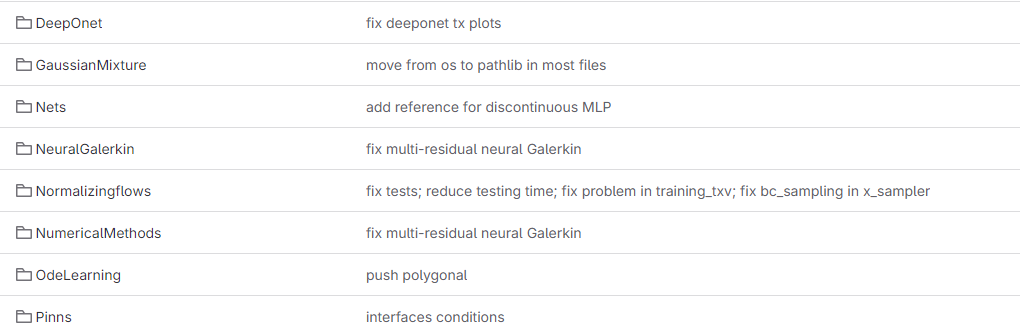
\includegraphics[width=8in]{images/ScimBa neural networks.png}  

\end{figure}


%~~~~~~~~~~~~~~~~~~~~~~~~~~~~~~~~~~~~~~~~~~~~~~~~~~~~~~~~~~~~~~

\newpage
\section{Creating the Docker container}
We both worked on creating the Dockerfile adding little by little the dependencies.
Creating a Docker container and image for the project offers these key advantages:
\begin{itemize}
        \item \textbf{Portability:} Run the project on any platform supporting Docker.
        \item \textbf{Reproducibility:} Recreate the exact same environment whenever needed.
        \item \textbf{Dependency Management:} Package all dependencies within the Docker image and avoid conflicts with other software on the host system.   
\end{itemize}
This Dockerfile creates a docker image with Feel++ as a base and installs the dependencies and libraries needed to run ScimBa in that environment.
It copies the public ScimBa repository into the 'scimba' folder and installs it.
We have also added command lines to automate script that let us run the program 'solve lap.py', that uses Feel++ libraries to solve a Laplacian problem and generates visuals.

\begin{lstlisting}[language=docker,caption={Dockerfile for Feel++, Scimba, and Python libraries.},frame=single, backgroundcolor=\color{gray!10}, basicstyle=\footnotesize,rulecolor=\color{blue}, framexleftmargin=3pt, commentstyle=\color{mygreen}, keywordstyle=\color{blue}]
# Start with the Feel++ base image
FROM ghcr.io/feelpp/feelpp:jammy

# Install system dependencies
RUN apt-get update && apt-get install -y \
    git \
   xvfb

# Install Python libraries
RUN pip3 install torch xvfbwrapper pyvista plotly panel ipykernel
    matplotlib

# Clone the Scimba repository
RUN git clone https://gitlab.inria.fr/scimba/scimba.git 
                    /workspaces/2024-m1-scimba-feelpp/scimba

# Install Scimba and its dependencies
WORKDIR /workspaces/2024-m1-scimba-feelpp/scimba
RUN pip3 install scimba

# Copy the xvfb script into the container
COPY tools/load_xvfb.sh /usr/local/bin/load_xvfb.sh
RUN chmod +x /usr/local/bin/load_xvfb.sh

# Set the script to initialize the environment
CMD ["/usr/local/bin/load_xvfb.sh"]

\end{lstlisting}



%~~~~~~~~~~~~~~~~~~~~~~~~~~~~~~~~~~~~~~~~~~~~~~~~~~~~~~~~~~~~~~
\newpage
\section{Methodology}
We decided to divide the work. Helya works on making a Feel++ solver and Rayen on a ScimBa one.

Given the Feel++ documentation and the Poisson class prototype that gives access to results from the Feel++ solver. Here's the work we did:
\subsection{Solving the PDE}

Create the right environment for using the CFPDE toolbox:
\begin{lstlisting}
import sys
import feelpp
import feelpp.toolboxes.core as tb

from tools.solvers import Poisson
sys.argv = ["feelpp_app"]
e = feelpp.Environment(sys.argv,
                       opts=tb.toolboxes_options("coefficient-form-pdes", 
                       "cfpdes"),
                       config=feelpp.globalRepository('feelpp_cfpde'))

\end{lstlisting}

Solving the Poisson equation with different parameters using the CFPDE toolbox

\begin{lstlisting}
P = Poisson(dim = 2)
P(h=0.08,  rhs='-1.0-1*y*x+y*y', g='0', order=1, geofile='geo/disk.geo',
    plot='2d.png')
P(h=0.1,  rhs='-1.0-2*y*x+y*y', g='0', order=1, plot='f2.png')

P = Poisson(dim = 2)
P(h=0.1, diff='{1.0,0,0,x*y}', rhs='1', plot='d1.png')
P(h=0.1, diff='{1+x,0,0,1+y}', rhs='1', plot='d2.png')

P = Poisson(dim = 3)
P(h=0.08, diff='{1,0,0,0,x+1,0,0,0,1+x*y}', g = 'x', rhs='x*y*z', 
geofile = 'geo/cube.geo', plot='3d.png') 

\end{lstlisting}

Adding solver flag when calling the Poisson Class.
\begin{lstlisting}
def __call__(self,
               h,                                       # mesh size 
               order=1,                                 # polynomial order 
               name='Potential',                        # name of the variable
               rhs='8*pi*pi*sin(2*pi*x)*sin(2*pi*y)',   # right hand side
               diff='{1,0,0,1}',                        # diffusion matrix
               g='0',
               geofile=None,
               plot=None,
               solver='feelpp'):                        # or solver ='scimba'
    """
\end{lstlisting}

%~~~~~~~~~~~~~~~~~~~~~~~~~~~~~~~~~~~~~~~~~~~~~~~~~~~~~~~~~~~~~~
\newpage


Solving using Feel++ and ScimBa

\begin{lstlisting}[language=Python,caption={},frame=single, backgroundcolor=\color{gray!10}, basicstyle=\footnotesize,rulecolor=\color{blue}, framexleftmargin=3pt, commentstyle=\color{mygreen}, keywordstyle=\color{blue}]

\begin{lstlisting}
P( rhs='-1.0-4*y*x+y*y', g='x', order=1, solver='feelpp')
P( rhs='-1.0-4*y*x+y*y', g='x', order=1, solver ='scimba')
\end{lstlisting}



\subsection{Computing L2 and H1 errors}
\subsubsection{Computing the errors}

This function iterates over a set of mesh sizes (`h`), computes the solution using a specified computational model, and appends the L2 and H1 errors to the dataframe.

\begin{lstlisting}[language=Python3,caption={},frame=single, backgroundcolor=\color{gray!10}, basicstyle=\footnotesize,rulecolor=\color{blue}, framexleftmargin=3pt, commentstyle=\color{mygreen}, keywordstyle=\color{blue}]

import plotly.express as px
from plotly.subplots import make_subplots
import itertools
import pandas as pd
import numpy as np

def runLaplacianPk(df,model,verbose=False):
    """generate the Pk case

    Args:
        order (int, optional): order of the basis. Defaults to 1.
    """
    meas=dict()
    dim,order,json=model
    for h in df['h']:
        m=laplacian(hsize=h,json=json,dim=dim,verbose=verbose)
        for norm in ['L2','H1']:
            meas.setdefault(f'P{order}-Norm_laplace_{norm}-error', [])
            meas[f'P{order}-Norm_laplace_{norm}-error'].append(m.pop(
                                f'Norm_laplace_{norm}-error'))
    df=df.assign(**meas)
    for norm in ['L2','H1']:
        df[f'P{order}-laplace_{norm}-convergence-rate']=
            np.log2(df[f'P{order}-Norm_laplace_{norm}-error'].shift() / 
                df[f'P{order}-Norm_laplace_{norm}-error']) / 
                np.log2(df['h'].shift() / df['h'])
    return df


\end{lstlisting}
\newpage

\subsubsection{Plotting the convergence rate}
Run the convergence analysis for different mesh sizes and polynomial orders. Generate and display a plot of convergence rates across mesh sizes for each polynomial order.

\begin{lstlisting}[language=Python3,caption={},frame=single, backgroundcolor=\color{gray!10}, basicstyle=\footnotesize,rulecolor=\color{blue}, framexleftmargin=3pt, commentstyle=\color{mygreen}, keywordstyle=\color{blue}]

def runConvergenceAnalysis(json,dim=2,hs=[0.1,0.05,0.025,0.0125],orders=[1,2],
                            verbose=False):
    df=pd.DataFrame({'h':hs})
    for order in orders:
        df=runLaplacianPk(df=df,model=[dim,order,json(dim=dim,order=order)],
                            verbose=verbose)
    print('df = ', df.to_markdown())
    return df

df=runConvergenceAnalysis(json=laplacian_json,dim=2,verbose=True)
def plot_convergence(df,dim,orders=[1,2]):
    fig=px.line(df, x="h", y=
        [f'P{order}-Norm_laplace_{norm}-error' for 
            order,norm in list(itertools.product(orders,['L2','H1']))])
    fig.update_xaxes(title_text="h",type="log")
    fig.update_yaxes(title_text="Error",type="log")
    for order,norm in list(itertools.product(orders,['L2','H1'])):
        fig.update_traces(name=f'P{order} - {norm} error - 
            {df[f"P{order}-laplace_{norm}-convergence-rate"].iloc[-1]:.2f}', 
                selector=dict(name=f'P{order}-Norm_laplace_{norm}-error'))
    fig.update_layout(
            title=f"Convergence rate for the {dim}D Laplacian problem",
            autosize=False,
            width=900,
            height=900,
        )
    return fig
fig=plot_convergence(df,dim=2)
fig.show()



\end{lstlisting}

%~~~~~~~~~~~~~~~~~~~~~~~~~~~~~~~~~~~~~~~~~~~~~~~~~~~~~~~~~~~~~~
\newpage

\section{Results}
\subsection{Generating visuals using Feel++}

Feel++ produces geometry files for either a 2D rectangle or a 3D box. The generated file is compatible with Gmsh, facilitating subsequent mesh generation and finite element analysis. The characteristic length $h$ controls the mesh resolution, and we define physical groups for boundaries and domains, which are crucial for setting boundary conditions and material properties in simulations. 
\newline

We define the method genCube within our class to generate the desired geometry:
\begin{lstlisting}[language=Python,caption={},frame=single, backgroundcolor=\color{gray!10}, basicstyle=\footnotesize,rulecolor=\color{blue}, framexleftmargin=3pt, commentstyle=\color{mygreen}, keywordstyle=\color{blue}]
def genCube(self, filename, h=0.1):
    """
    Generate a cube geometry following the dimension  self.dim
    """

    geo="""SetFactory("OpenCASCADE");
    h={};
    dim={};
    """.format(h, self.dim)
    
    if self.dim==2 :
        geo+="""
        Rectangle(1) = {0, 0, 0, 1, 1, 0};
        Characteristic Length{ PointsOf{ Surface{1}; } } = h;
        Physical Curve("Gamma_D") = {1,2,3,4};
        Physical Surface("Omega") = {1};
        """

    elif self.dim==3 :
        geo+="""
        Box(1) = {0, 0, 0, 1, 1, 1};
        Characteristic Length{ PointsOf{ Volume{1}; } } = h;
        Physical Surface("Gamma_D") = {1,2,3,4,5,6};
        Physical Volume("Omega") = {1};
        """
    with open(filename, 'w') as f:
        f.write(geo
\end{lstlisting}


%~~~~~~~~~~~~~~~~~~~~~~~~~~~~~~~~~~~~~~~~~~~~~~~~~~~~~~~~~~~~~~
\newpage

Generated 3D geometry and mesh viewed using gmsh:

\begin{frame}{}
    \begin{center}
        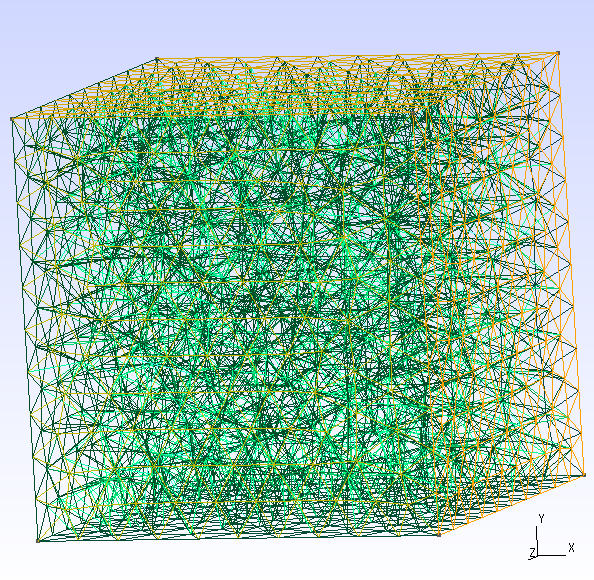
\includegraphics[width=2.2in\textwidth]{images/fppmsh.png}
    \end{center}
\end{frame}


 we illustrate the usage of the Poisson class for conducting finite element analysis, specifically focusing on solving the Poisson equation. The code snippet provided demonstrates the invocation of the Poisson class with specified parameters.
\newline

 We initiate the Poisson class instance P by specifying the dimension as 2:
\begin{lstlisting}
    P = Poisson(dim = 2)
    P(h=0.08,  rhs='-1.0-1*y*x+y*y', g='0', order=1, plot='f4.png')
\end{lstlisting}

Using the Poisson class, we solve the Poisson equation for a 2D area. Customizable parameters let us adapt the solver to different problems. This method helps analyze many phenomena governed by the Poisson equation, useful in science and engineering.

\begin{frame}{}
    \begin{center}
\includegraphics[width=0.35\textwidth]{images/fpp_pde_2d.png}
    \end{center}
\end{frame}


\begin{lstlisting}
    P = Poisson(dim = 3)
    P(h=0.08, diff='{1,0,0,0,x+1,0,0,0,1+x*y}', g = 'x', rhs='x*y*z', 
        geofile = 'geo/cube.geo', plot='3d.png')

\end{lstlisting}


\begin{frame}{}
    \begin{center}
        \includegraphics[width=0.35\textwidth]{images/fpp_pde_3d.png}
    \end{center}
\end{frame}    

%~~~~~~~~~~~~~~~~~~~~~~~~~~~~~~~~~~~~~~~~~~~~~~~~~~~~~~~~~~~~~~
\newpage

\subsection{Generating visuals using ScimBa}

We begin by defining the spatial domain \texttt{xdomain} using ScimBa's SpaceDomain module. In this case, we specify a two-dimensional domain using a square domain configuration spanning from $(0.0, 0.0)$ to $(1.0, 1.0)$;


Next, we create an instance of the Poisson equation \texttt{pde} in two dimensions, specifying the right-hand side (\texttt{rhs}) as well as the boundary condition function:

Finally, we execute the \texttt{Run\_laplacian2D} function, which solves the Poisson equation defined by \texttt{pde}:

\begin{lstlisting}
    xdomain = domain.SpaceDomain(2, domain.SquareDomain(2, [[0.0, 1.0], 
                                                        [0.0, 1.0]]))    
    pde = Poisson_2D(xdomain,  rhs='8*pi*pi*sin(2*pi*x)*sin(2*pi*y)', g='0')
    Run_laplacian2D(pde)
    
\end{lstlisting}

The visual representation generated by the above code snippet is depicted below:

\begin{frame}{}
    \begin{center}
        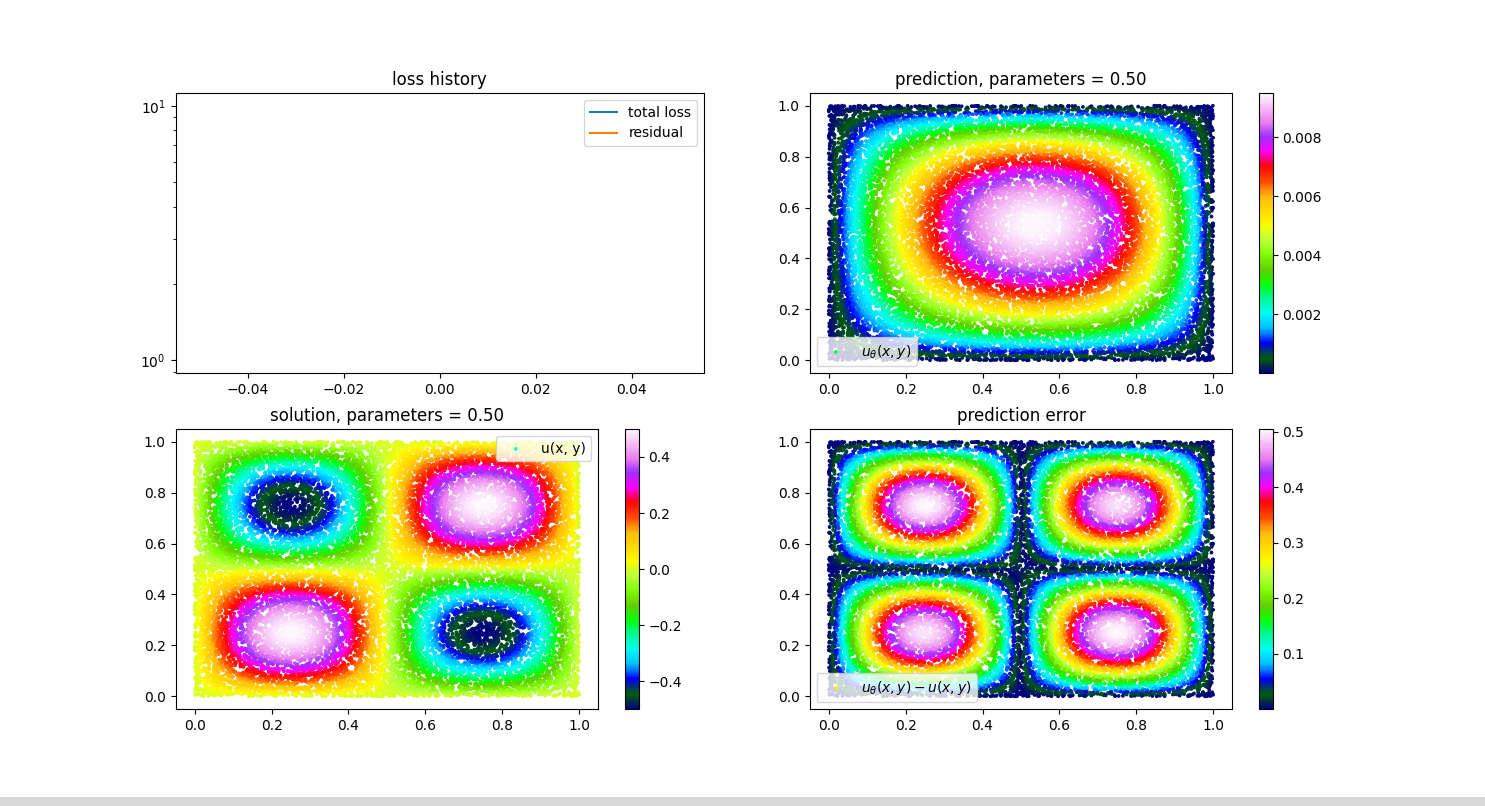
\includegraphics[width=0.9\textwidth]{images/scimbaplot1.png}
    \end{center}
\end{frame}


%~~~~~~~~~~~~~~~~~~~~~~~~~~~~~~~~~~~~~~~~~~~~~~~~~~~~~~~~~~~~~~

Then we initiate the visualization process by defining the spatial domain \texttt{xdomain} using ScimBa's SpaceDomain module. In this instance, we specify a two-dimensional domain utilizing a disk-based configuration with a center at $(0.0, 0.0)$ and a radius of $1.0$.

Subsequently, we create an instance of the Poisson equation \texttt{pde\_disk} in two dimensions, utilizing the disk-based spatial domain defined earlier.

Finally, we execute the \texttt{Run\_laplacian2D} function, which solves the Poisson equation defined by \texttt{pde\_disk}:

%~~~~~~~~~~~~~~~~~~~~~~~~~~~~~~~~~~~~~~~~~~~~~~~~~~~~~~~~~~~~~~
\newpage

\begin{lstlisting}
    xdomain = domain.SpaceDomain(2, domain.DiskBasedDomain(2, center=[0.0, 0.0],
                                                            radius=1.0))
    pde_disk = PoissonDisk2D(space_domain=xdomain)
    Run_laplacian2D(pde_disk)
    
\end{lstlisting}

The visual representation generated by the provided code snippet is presented below:

\begin{frame}{}
    \begin{center}
        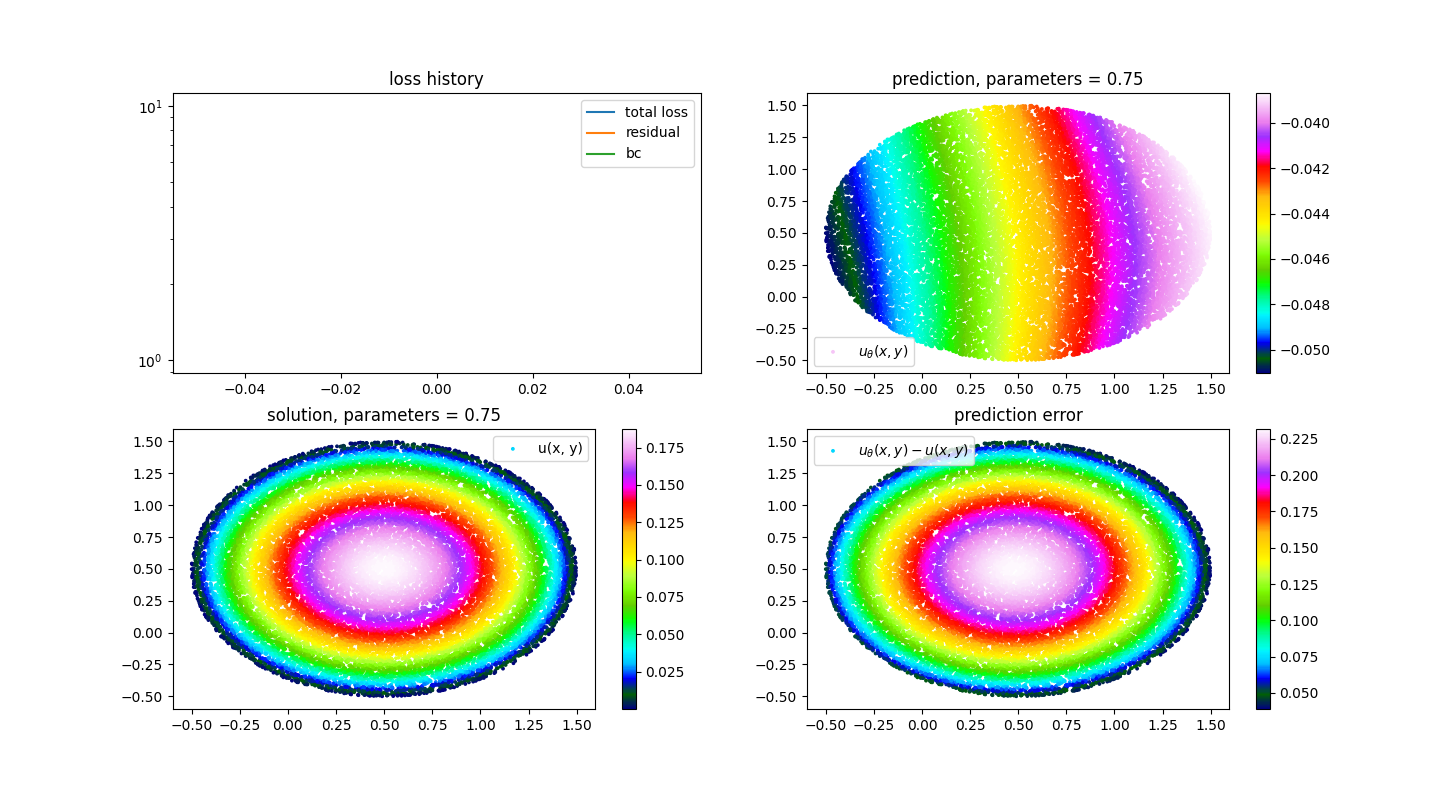
\includegraphics[width=0.9\textwidth]{images/scimbaplot2.png}
        \end{center}
\end{frame}

%~~~~~~~~~~~~~~~~~~~~~~~~~~~~~~~~~~~~~~~~~~~~~~~~~~~~~~~~~~~~~~
\subsubsection{Laplacian on ellipse mapping}

We initiate the computation and mapping process by defining the spatial domain \texttt{xdomain} using ScimBa's SpaceDomain module. In this instance, we specify a two-dimensional domain utilizing a disk-based configuration with a center at $(0.0, 0.0)$ and a radius of $1.0$. Additionally, we provide a custom mapping function \texttt{disk\_to\_ellipse} and its corresponding Jacobian function \texttt{Jacobian\_disk\_to\_ellipse}.

Next, we create an instance of the Poisson equation \texttt{pde} in two dimensions, utilizing the ellipse-based spatial domain defined earlier.

Finally, we execute the \texttt{Run\_laplacian2D} function, which computes the Laplacian on the ellipse and maps it using a neural network. Additionally, we set parameters \texttt{bc\_loss\_bool=True} to include boundary condition loss and \texttt{w\_bc=10} and \texttt{w\_res=0.1} to control the weight of the boundary condition and residual loss:
%~~~~~~~~~~~~~~~~~~~~~~~~~~~~~~~~~~~~~~~~~~~~~~~~~~~~~~~~~~~~~~
\newpage

\begin{lstlisting}[language=Python,caption={},frame=single, backgroundcolor=\color{gray!10}, basicstyle=\footnotesize,rulecolor=\color{blue}, framexleftmargin=3pt, commentstyle=\color{mygreen}, keywordstyle=\color{blue}]
    xdomain = domain.SpaceDomain(
        2,
        domain.DiskBasedDomain(
            2,
            [0.0, 0.0],
            1.0,
            mapping=disk_to_ellipse,
            Jacobian=Jacobian_disk_to_ellipse,
        ),
    )
    pde = Poisson_2D_ellipse(xdomain)
    Run_laplacian2D(pde, bc_loss_bool=True, w_bc=10, w_res=0.1)
    
\end{lstlisting}
\begin{frame}{}
    \begin{center}
        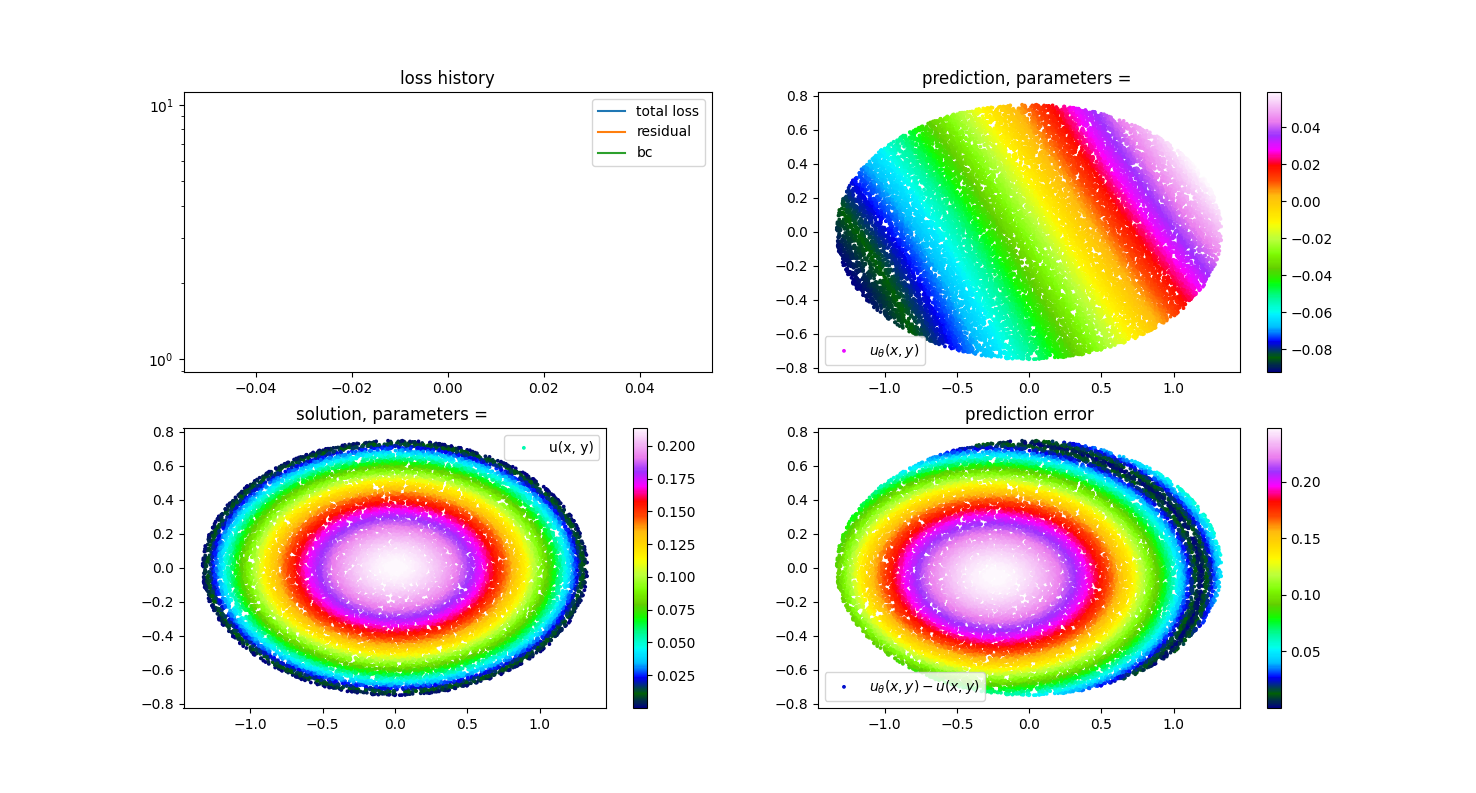
\includegraphics[width=0.9\textwidth]{images/scimbaplot3.png}
        \end{center}
\end{frame}

\subsubsection{Laplacian on potato mapping}

We also provide a custom mapping function \texttt{disk\_to\_potato} and its corresponding Jacobian function \texttt{Jacobian\_disk\_to\_potato}.

Next, we create an instance of the Poisson equation \texttt{pde} in two dimensions, utilizing the potato-shaped spatial domain defined earlier.

Finally, we execute the \texttt{Run\_laplacian2D} function, which computes the Laplacian on the potato-shaped domain and maps it using a neural network. We set parameters \texttt{bc\_loss\_bool=True} to include boundary condition loss and \texttt{w\_bc=10} and \texttt{w\_res=0.1} to control the weight of the boundary condition and residual loss.

\newpage
\begin{lstlisting}[language=Python,caption={},frame=single, backgroundcolor=\color{gray!10}, basicstyle=\footnotesize,rulecolor=\color{blue}, framexleftmargin=3pt, commentstyle=\color{mygreen}, keywordstyle=\color{blue}]
    xdomain = domain.SpaceDomain(
        2,
        domain.DiskBasedDomain(
            2,
            [0.0, 0.0],
            1.0,
            mapping=disk_to_potato,
            Jacobian=Jacobian_disk_to_potato,
        ),
    )
    pde = Poisson_2D_ellipse(xdomain)
    Run_laplacian2D(pde, bc_loss_bool=True, w_bc=10, w_res=0.1)

    
\end{lstlisting}
\begin{frame}{}
    \begin{center}
        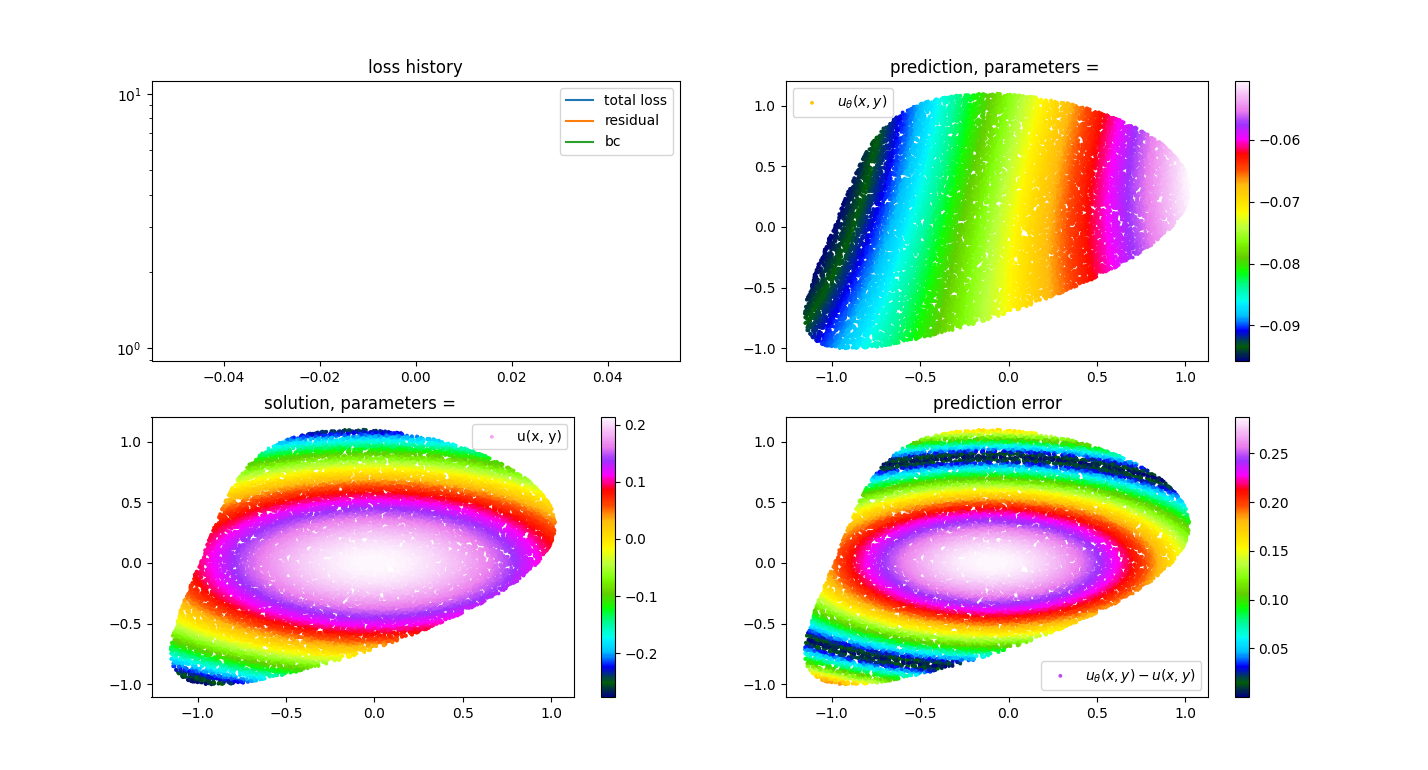
\includegraphics[width=5in\textwidth]{images/scimbaplot4.png}

    \end{center}
\end{frame}

This process allows us to analyze and visualize the behavior of the Laplacian on complex geometries, such as potato shapes, with the aid of neural networks. By including boundary condition loss and adjusting weights, we enhance the accuracy and control of the mapping process. This highlights the potential of combining numerical methods with machine learning techniques for solving and analyzing mathematical problems in scientific computing.
\newpage

\subsection{Comparing the visuals for a Laplacian problem }

This segment visualizes the Laplacian problem's solutions on a square domain. Using both the Feel++ and Scimba solvers, we assess the numerical accuracy and visual fidelity of solutions such as \( u = \sin(2\pi x) \sin(2\pi y) \), where the right-hand side \( f \) complements the exact solution's Laplacian.

\begin{lstlisting}[language=Python,caption={},frame=single, backgroundcolor=\color{gray!10}, basicstyle=\footnotesize,rulecolor=\color{blue}, framexleftmargin=3pt, commentstyle=\color{mygreen}, keywordstyle=\color{blue}]
# 2D on different domains
P = Poisson(dim = 2)

# for square domain
u_exact = 'sin(2*pi*x) * sin(2*pi*y)'
rhs = '8*pi*pi*sin(2*pi*x) * sin(2*pi*y)'

P(rhs=rhs, g='0', order=1, plot='f2.png', u_exact = u_exact)
P(rhs=rhs, g='0', order=1, solver ='scimba', u_exact = u_exact)
    
\end{lstlisting}


\begin{frame}{}
    \begin{center}
        \includegraphics[width=0.6\textwidth]{images/feel_exact.png}
        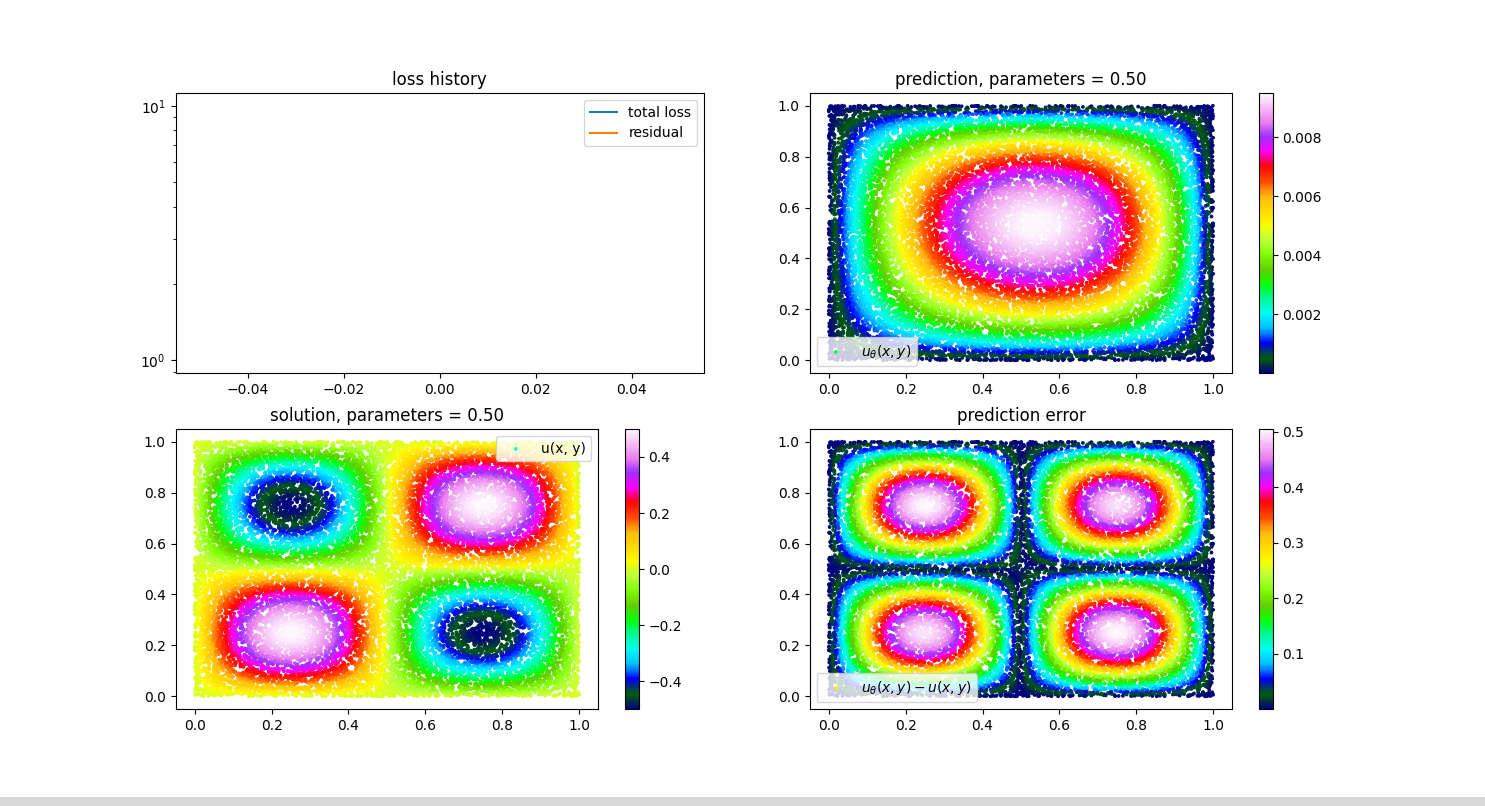
\includegraphics[width=0.7\textwidth]{images/scimbaplot1.png}

    \end{center}
\end{frame}

\newpage

In this part, the focus shifts to solving the Laplacian problem on a disk domain. The exact solution \( u = \sin(\pi(x^2 + y^2)) \) and its corresponding \( f \) are tailored to test the solvers' capabilities in more complex geometrical contexts.

\begin{lstlisting}[language=Python,caption={},frame=single, backgroundcolor=\color{gray!10}, basicstyle=\footnotesize,rulecolor=\color{blue}, framexleftmargin=3pt, commentstyle=\color{mygreen}, keywordstyle=\color{blue}]

# for disk domain
u_exact =  'sin(pi*(x*x + y*y))'
rhs = '4*pi*sin(pi*(x*x + y*y)) - 4*pi*pi*(x*x + y*y)*cos(pi*(x*x + y*y))'

P(rhs=rhs, g='0', order=1, geofile='geo/disk.geo', plot='2d.png', 
    u_exact = u_exact)
P(rhs=rhs, g='0', order=1, geofile='geo/disk.geo', solver='scimba', 
    u_exact = u_exact)

    
\end{lstlisting}

\begin{frame}{}
    \begin{center}
        \includegraphics[width=0.6\textwidth]{images/feel_disk.png}
        \includegraphics[width=0.7\textwidth]{images/scimba_disk.png}

    \end{center}
\end{frame}


%~~~~~~~~~~~~~~~~~~~~~~~~~~~~~~~~~~~~~~~~~~~~~~~~~~~~~~~~~~~~~~

\newpage

\subsection{Error convergence rate }

This is the Error convergence rate for a Laplacian problem using Feel++ tools. 
\begin{frame}{}
    \begin{center}
        \includegraphics[width=5in\textwidth]{images/newplot.png}
    \end{center}
\end{frame}


%~~~~~~~~~~~~~~~~~~~~~~~~~~~~~~~~~~~~~~~~~~~~~~~~~~~~~~~~~~~~~~

\newpage

\section{Conclusion}

Our ultimate goal is to streamline the process of solving complex mathematical problems and equations by harnessing the combined power of SimBa and Feel++. By integrating these two computational tools, we aim to contribute to two wide-ranged and ongoing projects.

ScimBa offers accessible tools for visualization, computation, and mapping of mathematical models, providing us valuable insights into the behavior of complex systems during our work in this project. Its flexibility and scalability aided us in understanding and interpreting Machine Learning methods.

Nevertheless, Feel++ provides a comprehensive framework for finite element analysis, offering customizable parameters for solving differential equations and simulating physical processes. 

By combining ScimBa's training capabilities with Feel++'s solver framework, we can leverage the strengths of both tools to solve problems more efficiently. 

This integration allowed us to perform comprehensive analyses, visualize results in meaningful ways, and gain deeper insights into both solvers.

\begin{frame}
The project demonstrates the use of the CFPDE toolbox, leveraging both Feel++ and ScimBa frameworks, for solving Poisson equations across two domains.The methodology involved setting up the environment, defining and solving Poisson problems, and generating visual representations of the results. The following key points summarize the outcomes:
\begin{enumerate}
    \item Environment Setup:
        \begin{enumerate}
            \item The Feel++ environment was initialized with the necessary configuration for using the CFPDE toolbox.
            \item The Poisson class prototype was effectively used to access and solve problems using the Feel++ solver.
        \end{enumerate}
        
    \item Solving Poisson Equations:
        \begin{enumerate}
            \item Poisson equations were solved for 2D domains with different parameters, including mesh size, diffusion matrices, and right-hand side functions.
            \item The solutions were computed using both Feel++ and ScimBa solvers.
        \end{enumerate}  

    \item Visualization:
        \begin{enumerate}
            \item Visuals generated using Feel++ displayed the solution on both 2D and 3D geometries, including complex shapes like disks and cubes.
            \item ScimBa also provided visuals for different domain configurations, such as square and disk-based domains.            
        \end{enumerate}  
  
\end{enumerate}
\item Challenges and setbacks:
    \begin{enumerate}
        \item Using time more appropriately with supervisors.
        \item Learning to use github in a more efficient way.
        \item Limited use examples. 
        \item Heavy files.          

    \end{enumerate} 
\item Remaining work:
    \begin{enumerate}
        \item Computing error convergence rates.
        \item Extracting solution directly from Scimba.
        \item Comparing convergence rates of both solvers. 
        \item Implement the wrapper on other PDEs, domains in higher dimensions.          

    \end{enumerate}   

\begin{frame}{}
    \begin{center}
        Thank You for your time and attention.
    \end{center}
\end{frame}

\end{frame}
%~~~~~~~~~~~~~~~~~~~~~~~~~~~~~~~~~~~~~~~~~~~~~~~~~~~~~~~~~~~~~~
\newpage

\part*{Bibliography}
\addcontentsline{toc}{part}{\textit{Bibliography}}
\bibliographystyle{unsrt}
\bibliography{References.bib}

\begin{thebibliography}{14}

\bibitem{feelpp}
Feel++. (n.d.). \textit{Finite method course}. Retrieved from \url{https://feelpp.github.io/cours-edp/#/}

\bibitem{pyfeelpptoolboxes}
Feel++. (n.d.). \textit{Python Feel++ Toolboxes}. Retrieved from \url{https://docs.feelpp.org/user/latest/python/pyfeelpptoolboxes/index.html}


\bibitem{sciml}
SciML. (n.d.). \textit{Laplacian 2D Disk}. Retrieved from \url{https://sciml.gitlabpages.inria.fr/scimba/examples/laplacian2DDisk.html}

\bibitem{scimba}
ScimBa. (n.d.). \textit{ScimBa Repository}. Retrieved from \url{https://gitlab.inria.fr/scimba/scimba}

\bibitem{feelppgithub}
Feel++. (n.d.). \textit{Feel++ GitHub Repository}. Retrieved from \url{https://github.com/feelpp/feelpp}


\bibitem{coupling}
Wikipedia. (n.d.). \textit{Coupling (computer programming)}. Retrieved from \url{https://en.wikipedia.org/wiki/Coupling_(computer_programming)}

\bibitem{scimba2}
SciML. (n.d.). \textit{ScimBa}. Retrieved from \url{https://sciml.gitlabpages.inria.fr/scimba/}

\bibitem{feelppdocs}
Feel++. (n.d.). \textit{Feel++ Documentation}. Retrieved from \url{https://docs.feelpp.org/user/latest/index.html}

\bibitem{Quick Start with Docker}
Feel++. (n.d.). \textit{Quick Start with Docker}. Retrieved from \url{https://docs.feelpp.org/user/latest/using/docker.html}


\end{thebibliography}




\end{document}

%Fin :)